\section{Méthodologie de mise en place du processus de data mining\cite{DMProces}}.
Au début des années 90, l'intérêt croissant  pour le data mining a mis en lumière l'absence d'une méthodologie pour la mise en place d'un processus de découverte de connaissances, applicable quelle que soit l'industrie visée ou l'outil utilisé. De ce besoin est née l'initiative \ac{CRISP-DM}.
\begin{figure}[ht]
	\centering
	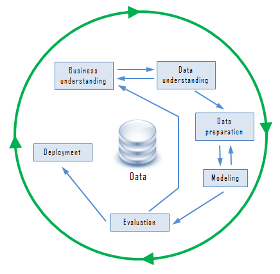
\includegraphics[width=0.5\textwidth]{fig/CRISP_tb.png}
	\caption[Short caption]{Data mining process model}
	\label{fig:imageCrisp}
\end{figure} 
A partir du processus de découverte de connaissances utilisé dans les premiers projets de data mining ,\ac{CRISP-DM} a défini et validé une méthodologie potentiellement applicable dans tous les secteurs de l'industrie. Elle permet de rendre les projets de data mining à grande échelle plus rapides, moins coûteux, plus fiables et surtout améliorer leur gestion. Cette méthodologie ne vise pas que les grands projets car même les petits projets de découverte de connaissances peuvent tirer profit de son utilisation.
Essentiellement, cette méthodologie fournit un aperçu du cycle de vie d'un projet de data mining. Elle identifie clairement les principales phases de ce processus au travers de tâches et des relations entre ces tâches. Même si le modèle ne le spécifie pas explicitement, il y a des relations possibles entre toutes les tâches en fonction des objectifs d'analyse et des données qui sont analysées.
Les six phases importantes du processus sont :
\begin{enumerate}
	\item \emph{La compréhension du problème métier} :  concerne la définition du problème d'analyse sur la base des objectifs métiers qui en sont à l'origine.
	\item \emph{La compréhension des données} :cette phase vise à déterminer précisément les données à analyser et à identifier la qualité des données .
	\item \emph{La préparation des données}: couvre les activités liées à la construction de l'ensemble précis des données à analyser à partir des données brutes. Ceci inclue le nettoyage des données, la sélection d'attributs, le choix des observations, etc.
	\item \emph{La modélisation }: est la phase consistant dans le paramétrage et le test de différentes techniques de data mining sur les données choisies, dans l'objectif d'optimisation du modèle ou des connaissances obtenues par ces techniques.
	\item \emph{L'évaluation }:vise à vérifier le modèle ou les connaissances obtenues afin de s'assurer qu'ils répondent aux objectifs formulés au début du processus. Elle contribue aussi à la décision de déploiement  du modèle ou, au contraire, de la nécessité que ce dernier soit reconstruit ou amélioré.
	\item \emph{Le déploiement }: est l'étape finale du processus de découverte de connaissances. Son objectif est de mettre la connaissance obtenue par la modélisation dans une forme adaptée et l'intégrer au processus de prise de décision. Le déploiement peut aller, selon les objectifs, de la simple génération d'un rapport décrivant les connaissances obtenue jusqu'à la mise en place d'une application spécifique permettant l'utilisation du modèle obtenu pour la prédiction des valeurs inconnues d'un paramètre d'intérêt.
\end{enumerate}

